\documentclass{article}

\usepackage[preprint]{nips_2018}
\usepackage[utf8]{inputenc} % allow utf-8 input
\usepackage[T1]{fontenc}    % use 8-bit T1 fonts
\usepackage{hyperref}       % hyperlinks
\usepackage{url}            % simple URL typesetting
\usepackage{booktabs}       % professional-quality tables
\usepackage{amsfonts}       % blackboard math symbols
\usepackage{nicefrac}       % compact symbols for 1/2, etc.
\usepackage{microtype}      % microtypography
\usepackage{graphicx}


\title{Ensuring Quality Conversations on Online Forums}


\author{%
  Luyu Chen\\
  \And
  Liang Huang\\
  \And
  Zhaorui Zeng\\
  \And
  Zhiming Xu\\
  \And Brandon Huang
}

\begin{document}
% \nipsfinalcopy is no longer used

\maketitle

\begin{abstract}
  Online forums can be toxic when users do not behave themselves. This toxicity degrades and corrupts thoughtful and respectful conversations. Hence, it becomes extremely important to detect such questions and deal with them properly. Our goal is to create a filter with deep neural networks to identify said toxicity and to prevent it from entering the conversation. In order to develop the filter, we will train a model with a Quora dataset composed of sincere and insincere questions. Our model mainly consists of a 2-layer LSTM as baseline, a TextCNN using one dimensional convolutional layer and a pre-trained language model BERT. We have trained them on a high-end GPU for hours. After training, we obtain parameters and can use them to run classification on ordinary hardware within a reasonable time. Both TextCNN and BERT have shown capable performance on insincere questions detection, especially BERT. The simple demonstration website, which could turned into a browser add-on, could potentially be used by various English based forums like Reddit and Quora.
\end{abstract}

\section{Introduction}
Nowadays, the internet has been a necessity for billions of netizens. Conversations through the Internet is so fast and convenient that people have relied on it for different situations such as professional discussion, idea sharing, chit-chat and reminders. Online forums have become one of the most important channels where people can meet new people, check for information, and share ideas. However, unfriendly forums with unrelated topics might destroy the conduciveness of such environments. Given the anonymity, the ever-changing of the online environments, and the difficulty in interpreting the nuances in the sentences, it is hard to track for unfriendly comments and questions. In the past, people who are in charge of the forums could check individually or encourage users to report those questions. However, it could be very subjective and require heavy manpower. In order to predict whether a question or comment is insincere, we have tried to collect language sets from Facebook, Twitter, Quora and Reddit. Luckily we also obtained 1.3 million quora questions labeled with insincere or not. This is large enough to train different kinds of deep neural networks. 

We have developed a baseline model as an important reference. The baseline model is trained using a two-layer LSTM, followed by a sigmoid output layer. Thus, given an input sequence, the LSTM would produce a representation sequence and average out into a fixed-length sentence representation. The output function is designed to be a sigmoid function because the question could be approached as a binary classification problem. That is, the problem is either friendly or unfriendly. For the baseline model, the test  accuracy reaches 94.3\%. For the reference of readers, 95\% seems like a great outcome. It is worth noticing that there are more sincere questions marked as 0 than insincere ones. Therefore, it is safe to argue that the model is valid with a test accuracy greater than 95%.

With the help of deep learning models, we managed to train our model with the TextCNN and BERT. TextCNN and BERT are based on two different types of neural network, that is, convolutional neural network and recurrent neural network.  Details are elaborated in the following section. Furthermore, we will be introducing our data source and how we preprocessed our data to fit into our models in the second section, our model with limitations in the third section, and future usage in the fourth section.

\section{Data}
We collected genuine question pairs from Quora as the training data set and collected computer-generated question pairs as the test data set as shown in the Table~\ref{tab:data}. 

\begin{table}[h!]
	\centering
	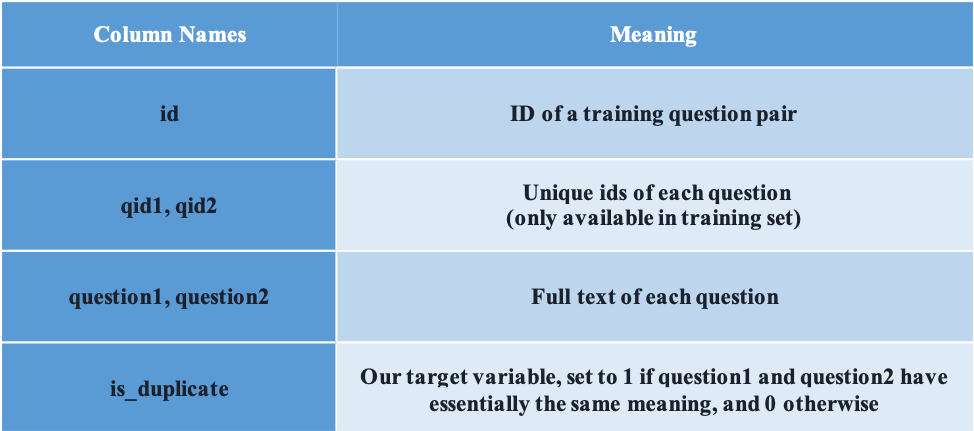
\includegraphics[scale=0.8]{data.png}
	\caption{Features in Our Dataset}
	\label{tab:data}
\end{table}


Embedding was used in our model. We checked the numbers and percentages of the missing values within the data set. It turned out that there were extremely few missing values in the data set. Thus, we only need to drop them after making sure that the positions and missing reasons for the data points are trivial. 

We processed our data to fit into our models. First, we cleaned up irregularities like punctuations and stop words, changed all words into lower-case, and got stem words. This is because text data often has many inconsistencies that will cause errors in the algorithms. For example, ‘Apple’, ‘APPLE’, ‘@Apple’ and ‘apple’ all have the same meaning but are considered different as words. After that, we checked the summary of the distribution of our data to make sure irregular values do not exist. Next we used a word as a token and created a dictionary based on the training set with the words segmented. This is important because the meaning of text generally depends on the relations of words in the text. Because the questions have different lengths, they cannot be directly combined into mini-batches. Here we fix the length of each comment to 200. Then we created data iterators for training. Depending on the language and intended use, iterators will provide additional operations or exhibit different behaviors. The primary purpose of an iterator is to allow us to process every element of a container while isolating the user from the internal structure of the containers.

\section{Model}
\subsection{Model Construction}

In order to build our model, we first consider simple RNN structure with LSTM cells. We choose glove 300d trained on Wikipedia as word embeddings. After converting samples in our data into vectors, we feed them into two layer of LSTM cells, and connect the outputs of the second layer to a final dense layer to produce two dimension classification of this sample. The method is quite straightforward, but it does not prove to be useful. After training on 700k labeled samples, we have achieved 94\% accuracy. However, since the positive samples take over ~95\% of whole training data, we suspect that this vanilla model in fact does not really distinguish good questions from bad ones. Hence, we use the 200k held-out data to verify our assumption. Of all ~10k bad samples, it only captures very few of them. Therefore, we switch to more complicated models. 

For efficient training, we deploy TextCNN as our new model, which treats text information alike image information. After vectorizing the word, since each word corresponds to a one dimension array, a sentence is encoded as a two dimension matrix. Intuitively, we can do convolution on this matrix as we typically do to an image. However, we must pay attention that truncated word vector do not make much sense. Hence the convolution layer should on one dimension, taking all the entries of one particular word's embedding into account, and on the other dimension, including one or several continuing words in a sample to abstract their combining meanings. We use multiple such convolution layers to capture the meaning of different word bags and connecting the results to a final dense layer to obtain the predictions. TextCNN proves to be more useful than simple two-layer LSTM, with an increasing of accuracy to ~95\%, indicating that it is able to recognize some insincere contents. 

\begin{figure}[h!]
	\centering
	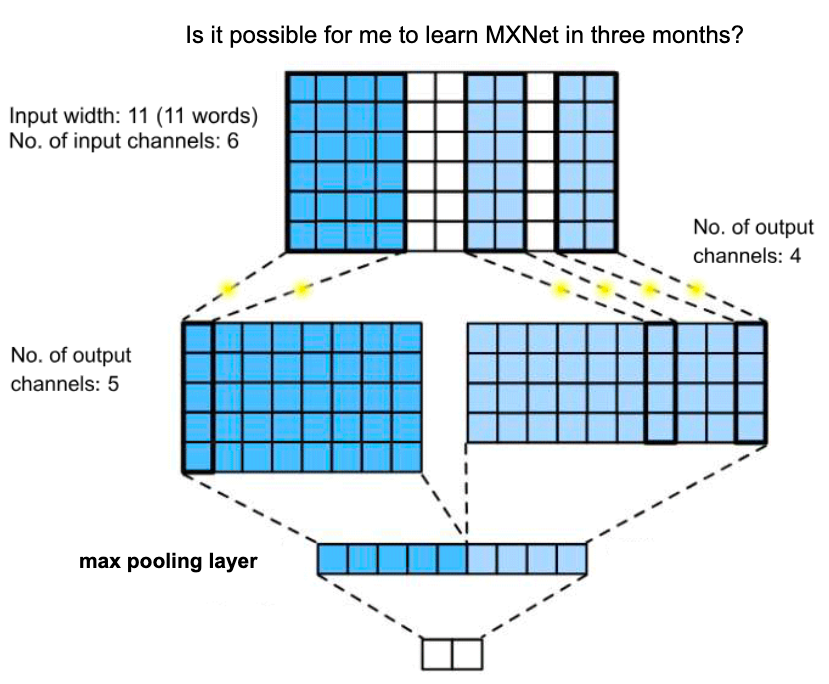
\includegraphics[scale=0.4]{flow.png}
	\caption{TextCNN Classifier}
	\label{fig:flow}
\end{figure}

Apart from these two models, we exploit BERT for pretraining and feature extraction, which uses multiple layers of position-wise feed forward network multi-head self-attention to capture features in language. Due to computation power and memory limit, we choose to use BERT base 768d trained on Wiki texts as our encoder. After tokenizing and feeding our samples into BERT, it will produce a 768d vectors representing the extracted information, which is then connected to the final output layer to obtain the binary predictions.

\begin{figure}[h!]
	\centering
	\includegraphics[scale=0.5]{bert.png}
	\caption{BERT Classifier}
	\label{fig:bert}
\end{figure}

\newpage
\subsection{Demonstration}
The website used for demonstration is run on free-tier AWS service site. It is implemented using prediction interfaces provided in both models and create embeddings for each sentences based on the vocabulary built for each model, as shown in Figure~\ref{fig:demo1}.

\begin{figure}[h!]
	\centering
	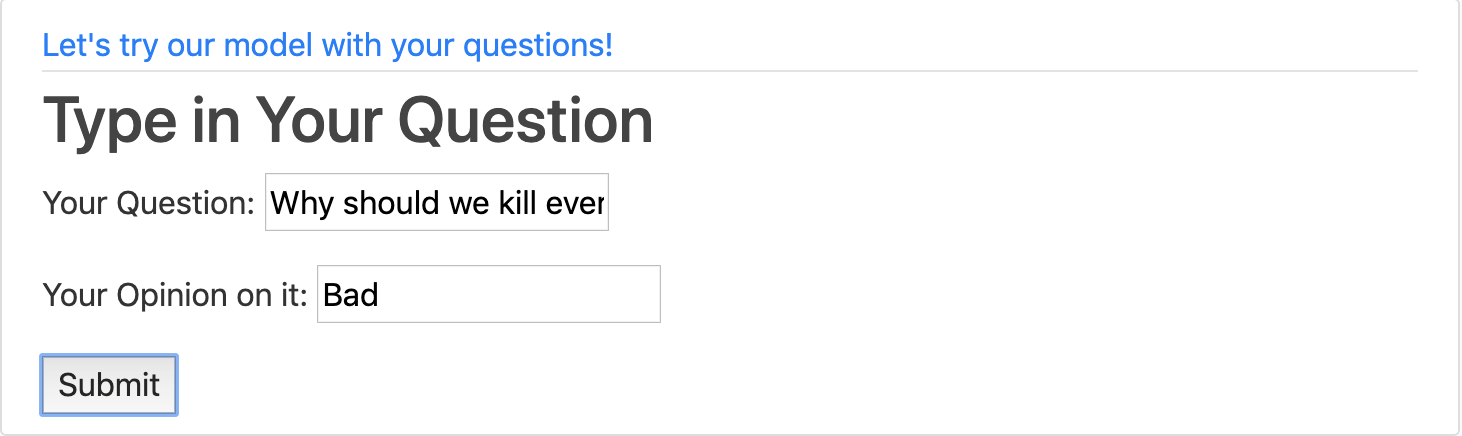
\includegraphics[scale=0.5]{demo1.png}
	\caption{Demonstration Website Key-in Page}
	\label{fig:demo1}
\end{figure}

In our demonstration, we showcased a couple of odd limitations as well as some possible questions. The first question we demonstrated was ‘Should we kill all human beings’ which produced a bad question from both our BERT and TextCNN models, as shown in Figure~\ref{fig:demo2}. However, if we change the word ‘all’ in the sentence to ‘some’, our machine reports the question as valuable. This generalization problem is a limitation that we can tackle by reducing the dataset so that the deep learning algorithm can learn by itself. 

\begin{figure}[h!]
	\centering
	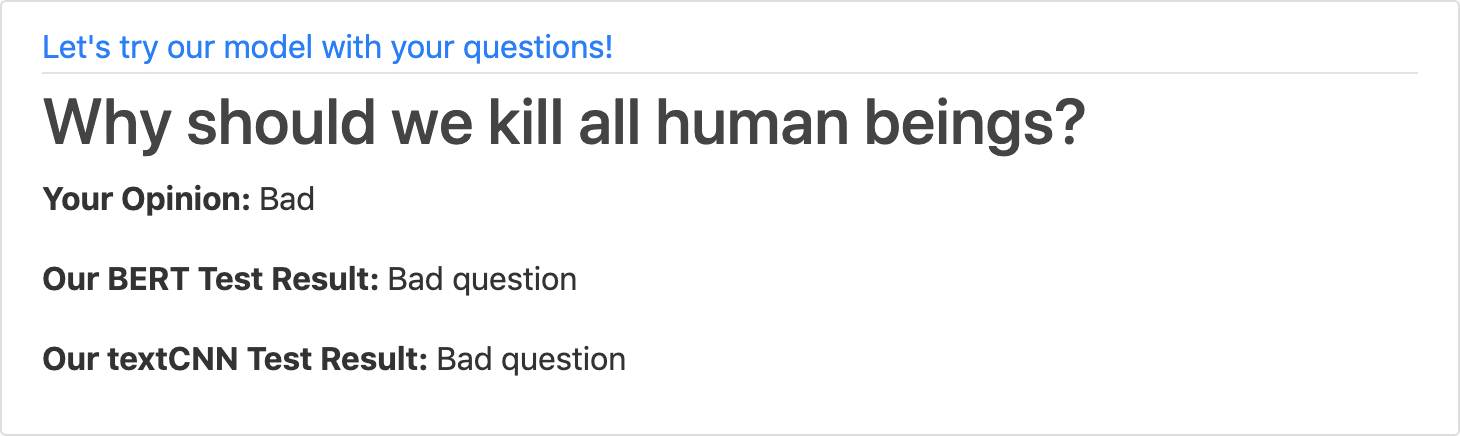
\includegraphics[scale=0.5]{demo2.png}
	\caption{Demonstration Website Result Page}
	\label{fig:demo2}
\end{figure}

There are also cases where the BERT and TextCNN models produce opposing answers. Usually, the TextCNN model produces better answers for generalization questions while BERT fails to recognize a generalized question. A possible solution for this problem is to have multiple models with different volumes of datasets to best determine if the question is valuable or not valuable. We can use the average of multiple models to predict an accurate analysis for these questions.

\section{Performance}
As mentioned in the introduction section, the model is valid only when the test accuracy is greater than or equal to 95\% considering that of the large portion of sincere questions. It could be concluded directly from the performance metrics that as a baseline model, a 2-layer LSTM is doing nothing more than guessing while TextCNN and BERT shows effectiveness. BERT outperforms TextCNN with respect to the test accuracy and reached a test accuracy of 98\%. We can view the result in Table~\ref{fig:acc}

\begin{table}[h!]
	\centering
	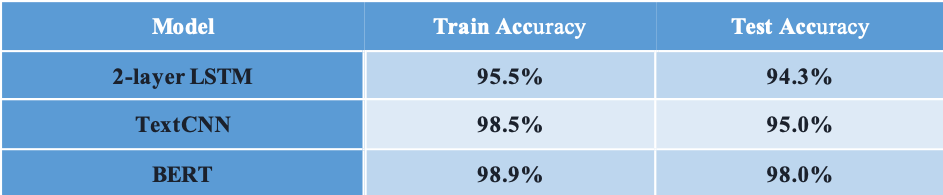
\includegraphics[scale=0.8]{acc.png}
	\caption{Performance of different models}
	\label{fig:acc}
\end{table}

It is interesting that for TextCNN and BERT, few unexpected patterns have been learned by the two deep neural networks. The first one is the question mark. Oftentimes, the result shows a contradiction with or without a question mark. It is reasonable to make the hypothesis that because more than 99\% of the questions that were fed into the networks are with a question mark, the networks learn a specific pattern with the question marks. The second one is more obvious with examples. As shown in the demo, both BERT and TextCNN learn to identify the quantifiers like ‘all’, ‘some’, ‘everyone’, ‘someone’, e.t.c. It is an unexpected pattern that may greatly contribute to the accuracy for insincere question detection. One paired example is ‘Should we kill all human being?’ and ‘Should we kill some of the human being’. It is quite reasonable for the former one to be detected as ‘insincere’ as it has a tone of ‘anti-society’. The latter one could be a valuable discussion for death penalty. It could not be told from just the title. More information may be used for further identification with the description of a question at online forums.

TextCNN and BERT has its own limitations. For TextCNN, the limitations show mainly in the test accuracy. It falls far behind BERT. While it seems that BERT outperforms all other models, its limitations mainly reside in the inefficiencies of the training. First the training process takes a super long time. That means that if it is intended to adapt to a new scenario, probably not quora but some foreign language forums, days could be needed to train a new model.  Along with the training time is the memory consumption - it takes around 5 gigabytes to store the parameters.

In addition, the nature of human language proposed certain limitations. For example, the ambiguity of language itself. The following is the distributions of tags added by 17 distinct human beings for five questions: ‘What is the best pesticide to commit suicide in India?’. ‘Is a decisional tree better than logistic regression?’ , ‘Is it possible to learn Hadoop in three months’, “Why don't India start a War with Pakistan ? They Kill our Soldiers.’ and  ‘What is the gayest country in the world?’. Among them, only the second and third one are recognized as sincere by BERT. However, humans hold different opinions even for the second question. The fact also provides potential improvements in the future - adding the human-made tags to the loss function of the neural networks. 



\section{Improvements and Future Usage}
To deal with the unexpected learned pattern of our BERT model, we try different solutions. First, we introduce some "noises", which are comments from Reddit to help the model less concentrate on the specially order of interrogative sentences. The experiment includes thousands of such comments as samples. Our result shows that this method does not have too much effect, and the model still often fails to detect an insincere declarative sentences as before. It is probably because the newly introduced samples only take up a small portion of training data and do not have a large influence on our model. Then we try to remove the question mark in training samples, which reduces accuracy of 0.3\% but proves to be more helpful for generalizing this model to common sentences. The accuracy for detecting such samples increase largely.

In order to evolve the capabilities and versatility of TextCNN and BERT models,  we can also add the analysis of sentences to our models. While Quora's initial contact is based off of a question, all comments that come after are in the format of sentences. Therefore, having sentence analysis is crucial to our model having full coverage of any online forum, post, or blog. A possible product that we can incorporate this functionality is CloudFlare. CloudFlare provides websites with spam protection and constant caching. By implementing deep learning models within CloudFlare, CloudFlare's users can create a more valuable platform based off of meaningful comments. 

From there, we want to incorporate spoiler detection for online forums like Reddit. For example, when there is a Game of Thrones post with the tag ‘No Spoilers’, the system flags that and starts filtering out comments that have spoilers. For the training dataset, we can use multiple Game of Thrones Wikipedias so that the model has real-time qualifiable data. Furthermore, we need an incredible amount of processing power for this because these type of threads are usually posted within seconds of an episode airing. Another use case for this feature is for sports games so that people who have not watched the game can safely browse the internet without the fear of spoiling the game. Another type of internet company that can utilize this technology is any internet browser company. This piece of technology would allow them to filter out custom content for customer profiles of internet users.

The last step in our evolution is to incorporate forum topic specific filtering. A sample reddit forum topic may be ‘What is the best way to waste your life?’ As you can probably tell, many of the comments would be seen as generally malicious. However, because the forum topic purpose is to generate these type of answers, the model has to be able to realize this and filter accordingly to the topic. This feature is crucial to the integrity of any forum, blog, or post. Because most of these topics have been posted before, we can scrape the web for similar topics and use those threads as training datasets. This functionality would ultimately require a mass amount of data which is why it is the last step of our evolutionary process. 

\section{Conclusion}
We were inspired by multiple forums to create a filter for the forums. Throughout this process, we realized the endless possibilities and potentials of our technology. Not only can the technology be leveraged by online forums, but it can also be leveraged internet browsers (IE, Chrome). Our filtering system can power the user profile and content delivery of these internet companies. For example, a parent can set a child parameter on an internet browser and the browser uses our filtering technology to detect any content that are out of those parameters. 

As the internet progresses, we believe that Machine Learning and Deep Learning can make bountiful leaps across multiple platforms on the web. Forums can moderate themselves by incorporating deep learning so that it can learn about their user patterns and behaviors. Ultimately, this would make the internet a better and safer place. 


\section*{References}

\small

[1] Pennington,\ Jeffrey, Richard Socher, \& Christopher Manning.\ (2014) {\it Glove: Global vectors for word representation.} Proceedings of the 2014 conference on empirical methods in natural language processing (EMNLP).

[2] Kim, Y. (2014). {\it Convolutional neural networks for sentence classification.} arXiv preprint arXiv:1408.5882.

[3] Devlin \& Jacob, et al. \ (2018) {\it Bert: Pre-training of deep bidirectional transformers for language understanding.} arXiv preprint arXiv:1810.04805.


\section*{Contributions}
Conclusion of contributions: The topic is chosen by Zhaorui. Everyone in this team have made reasonable contributions. The project is originally divided into three parts: TextCNN (Zhaorui, Brandon), BERT (Luyu, Zhiming) and website (Liang). Everyone finished their job. The ‘academic’ leader is Zhiming, who has an interest in doing NLP in the future. 

\textbf{Brandon}: Collaborated with ZhaoRui on TextCNN model, Ran multiple AWS test, Presented 4.5 min/ 10 min presentations, Contributed and proofread content for both Mid-Semester and Final Report.  

\textbf{Luyu}: Collaborated with ZhaoRui on TextCNN predict function; Collaborated with Zhiming on BERT. Write APIs for websites with Zhiming. Present at Mid-Semester. Contributed to a large portion of contents for two presentations/reports.

\textbf{Zhaorui}: Identified our project topic; Coded Python classes to read raw text data from source files and store them as list-of-list objects; Built TextCNN model and made it a tool for prediction with Brandon and Luyu. Presented at final presentation. 

\textbf{Liang}: Collaborated with Zhiming for the demonstration website and designed the PowerPoint slides for both the introduction and the final presentation. Contributed to the final presentation. Collaborated with Luyu for the final report drafting and formatting. 

\textbf{Zhiming}: Experiment on LSTM to obtain preliminary results. Prepare for proposal slides, and present at midterm. Discuss new ideas and models to improve our model, i.e., TextCNN and BERT with other teammates. Adjust BERT pretraining to suit our task, train it and write the interface for demonstration. Help Luyu and Liang maintain demo website and integrate full results into it. Write about model and usage limitation for final slides. Experiment on limitation and propose potential methods to resolve them.

\end{document}
